%----------------------------------------------------------
% report_temp.tex
% v1.0
% 2022/10/28
% by Carlos Rodríguez - Pardo, 2023, Universidad Carlos III de Madrid
% ----------------------------------------------------------

\documentclass{wsdcr}
\usepackage[spanish]{babel}
\usepackage{float}
\usepackage{caption}
\usepackage{subcaption}


\title{Análisis Avanzado de Datos - Práctica Final}
\author{Dario, Muñoz Muñoz (NIA: 100405982)}
\date{\today}

\begin{document}

\maketitle

\section{Introducción}
Spotify es una plataforma de streaming de música que ofrece a sus usuarios acceso a millones de canciones de diversos géneros y épocas. Para mejorar la experiencia de los usuarios, Spotify utiliza la inteligencia artificial (IA) para analizar las características acústicas y la popularidad de las canciones, y así poder ofrecer recomendaciones personalizadas, listas de reproducción y radios. El conjunto de datos Spotify Dataset 1921-2020, 600k+ Tracks recoge información sobre más de 600 mil canciones publicadas entre 1921 y 2020, incluyendo datos como el nombre, los artistas, la fecha de lanzamiento, la duración, la presencia de contenido explícito y varios atributos acústicos como la danzabilidad, la energía o el tempo \cite{SpotifyDataset}. En este trabajo se pretende explorar este conjunto de datos utilizando dos tipos de aprendizaje automático: el supervisado y el no supervisado. El primero se basa en utilizar datos etiquetados para entrenar un modelo que pueda predecir la salida o la clase de nuevos datos. El segundo se basa en utilizar datos sin etiquetar para descubrir patrones ocultos o agrupaciones en los datos. El objetivo es aplicar ambos tipos de aprendizaje para obtener información relevante sobre las canciones y sus características.

Para el aprendizaje supervisado, nos centraremos en predecir la popularidad de las canciones a partir de sus atributos acústicos. La popularidad es un valor numérico entre 0 y 100 que indica el grado de éxito o reconocimiento de una canción en Spotify. Para dar una mayor vision a nuestro objetivo tenemos este trabajo \cite{PredictingPopularityonSpotify} en el que el autor intenta predecir la popularidad pero sin conseguir buenos resultados.

Para el aprendizaje no supervisado, nos centraremos en agrupar las canciones por su danzabilidad a partir de sus atributos acústicos. La danzabilidad es una categoría que describe el grado de facilidad para bailar la canción. Otro proyecto que realiza algo parecido seria el siguiente: Spotify Danceability and Popularity Analysis using SAP \cite{SpotifyAnalysis}

\section{Dataset}

El dataset escogido es de Yamac Eern AY y se llama "Spotify Dataset 1921-2020, 600k+ Tracks". Contiene 600 mil canciones lanzadas entre 1921 y 2020. Este dataset puede ser usado para tareas de aprendizaje supervisado y no supervisado, como clasificación, regresión o agrupamiento. El dataset contiene dos archivos, uno llamado "tracks.csv" tiene 20 columnas con los siguientes datos:

\begin{itemize}
    \item \textbf{id}: el identificador único de cada canción en Spotify (cadena alfanumérica).
    \item \textbf{name}: el nombre de la canción (cadena de texto).
    \item \textbf{popularity}: el nivel de popularidad de la canción en una escala de 0 a 100 (número entero).
    \item \textbf{duration\_ms}: la duración de la canción en mili segundos (número entero).
    \item \textbf{explicit}: si la canción tiene contenido explícito o no (0 = no, 1 = sí) (número binario).
    \item \textbf{artists}: los artistas que participan en la canción (lista de cadenas de texto).
    \item \textbf{id\_artists}: los identificadores únicos de los artistas en Spotify (lista de cadenas alfanuméricas).
    \item \textbf{release\_date}: la fecha de lanzamiento de la canción en formato YYYY-MM-DD (cadena de texto).
    \item \textbf{danceability}: el grado de facilidad para bailar la canción en una escala de 0 a 1 (número decimal).
    \item \textbf{energy}: el nivel de energía e intensidad sonora de la canción en una escala de 0 a 1 (número decimal).
    \item \textbf{key}: la tonalidad musical principal de la canción en una escala cromática estándar que va del 0 al 11, donde el 0 es Do y el 11 es Si (número entero).
    \item \textbf{loudness}: el nivel promedio del volumen sonoro en decibelios (dB) durante toda la canción (número decimal negativo o cero).
    \item \textbf{mode}: el modo musical principal de la canción, donde el 0 es menor y el 1 es mayor (número binario).
    \item \textbf{speechiness}: el grado en que se habla o se canta durante la canción en una escala del 0 al 1 (número decimal).
    \item \textbf{acousticness}: el grado en que se usan instrumentos acústicos o eléctricos durante la canción en una escala del 0 al uno (número decimal).
    \item \textbf{instrumentalness}: el grado en que se usan instrumentos musicales o voces humanas durante la canción en una escala del cero al uno (número decimal).
    \item \textbf{liveness}: el grado en que se percibe que hay público presente durante la grabación o reproducción de la canción en una escala del cero al uno (número decimal).
    \item \textbf{valence}: el grado en que se transmite un sentimiento positivo o negativo durante la canción en una escala del cero al uno (número decimal).
    \item \textbf{tempo}: el ritmo promedio expresado como las pulsaciones por minuto(BPM) durante toda la canción(número decimal).
    \item \textbf{time\_signature}:el número promedio expresado como fracciones simples(4/4 ,3/4 , etc.)de las pulsaciones por compás musical durante toda la canción(número entero).
\end{itemize}

Este dataset es muy útil para analizar las tendencias musicales a lo largo del tiempo y las preferencias del público. También puede servir para generar recomendaciones personalizadas o crear nuevas composiciones musicales basadas en los atributos acústicos.

\section{Análisis del Dataset}

Para realizar un buen análisis de datos del Dataset, primero mostraremos la matriz de correlación y la explicaremos. La matriz de correlación nos permite ver la relación lineal entre las variables numéricas del Dataset. Algunas de las correlaciones más destacadas son:

\begin{itemize}
    \item La variable loudness tiene una alta correlación positiva con la variable energy (0.76), lo que indica que a mayor intensidad sonora, mayor nivel de energía percibida en las canciones.
    \item La variable valence tiene una moderada correlación positiva con la variable danceability (0.53), lo que sugiere que a mayor grado de positividad o alegría expresada en las canciones, mayor facilidad para bailarlas.
    \item La variable acousticness tiene una alta correlación negativa con la variable energy (-0.72) y una moderada correlación negativa con la variable loudness (-0.52), lo que implica que a mayor presencia de elementos acústicos en las canciones, menor nivel de energía y menor intensidad sonora.
\end{itemize}

Estos resultados nos permiten conocer mejor las características y relaciones entre las variables del Dataset y nos ayudan a entender mejor las características de las canciones del Dataset y a identificar posibles patrones o tendencias.

\begin{figure}[H] 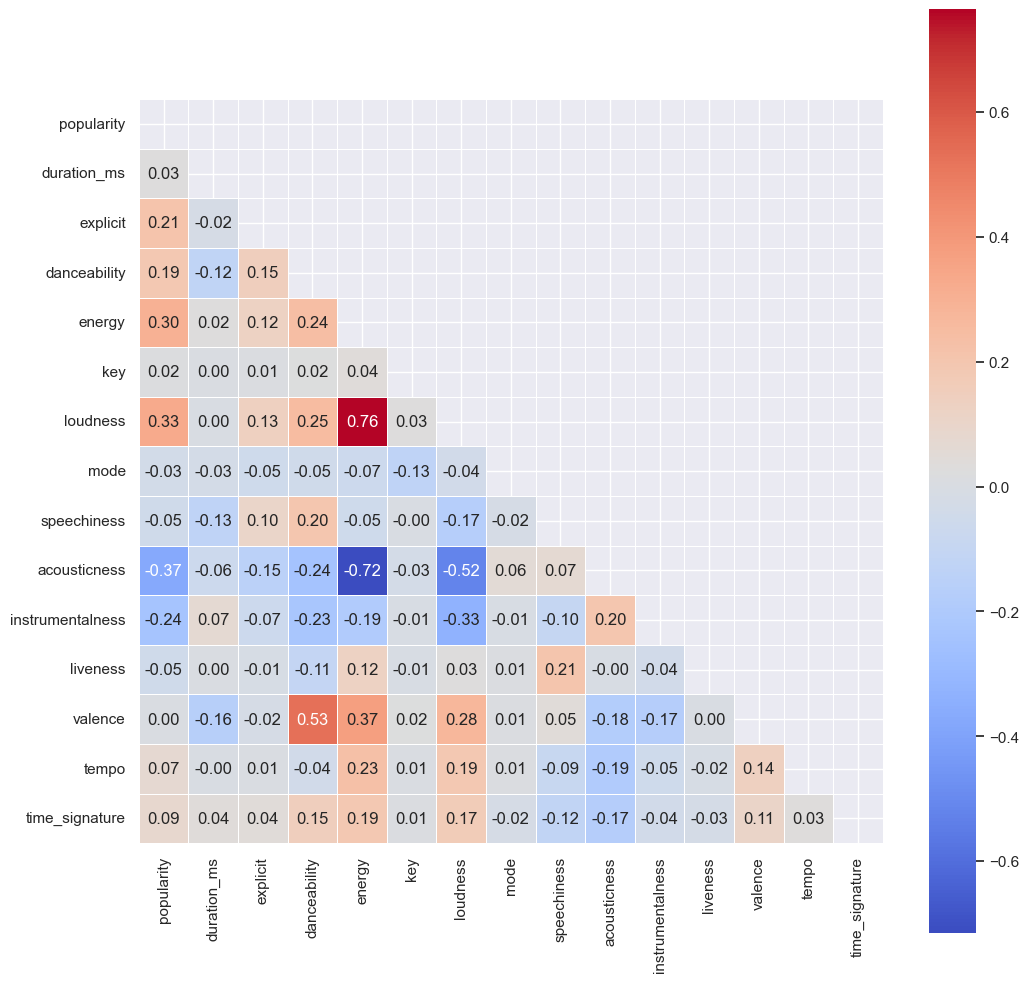
\includegraphics[width=\columnwidth]{images/matriz_correlacion.png} \caption{Matriz de correlación} \label{fig:matriz_correlaccion} \end{figure}

También para analizar el dataset realizaremos un histograma en la \figurename{\ref*{fig:histogramas}}, de cada variable que vamos a predecir, es decir popularidad y danzabilidad. Esto para ver cómo están distribuidas estas variables en el dataset.


\begin{figure}[H] 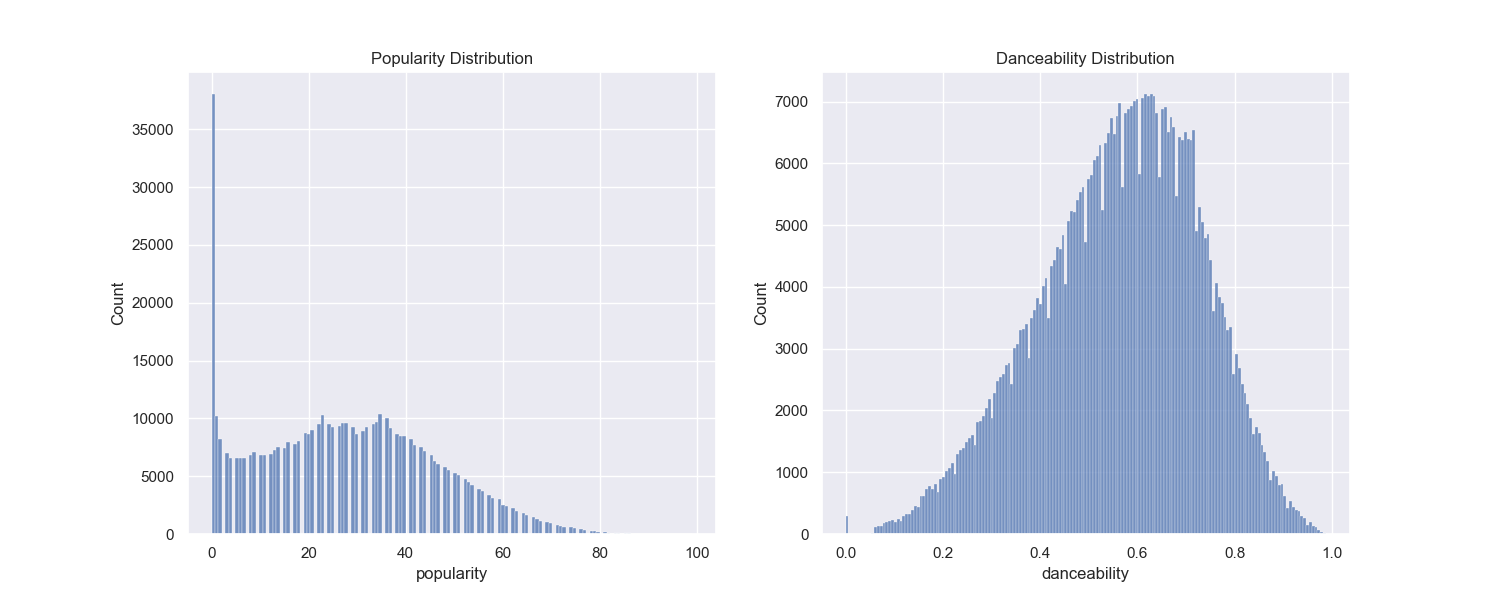
\includegraphics[width=\columnwidth]{images/histogramas.png} \caption{Histograma de popularidad y danzabilidad} \label{fig:histogramas} \end{figure}

Asimismo se ha realizado una comparación entre variables representativas como son la popularidad y la intensidad sonora, en la \figurename{\ref*{fig:relacion popularidad e intensidad sonora}}. en este se puede ver que tienen más popularidad las canciones con mayor intensidad sonora.

\begin{figure}[H] 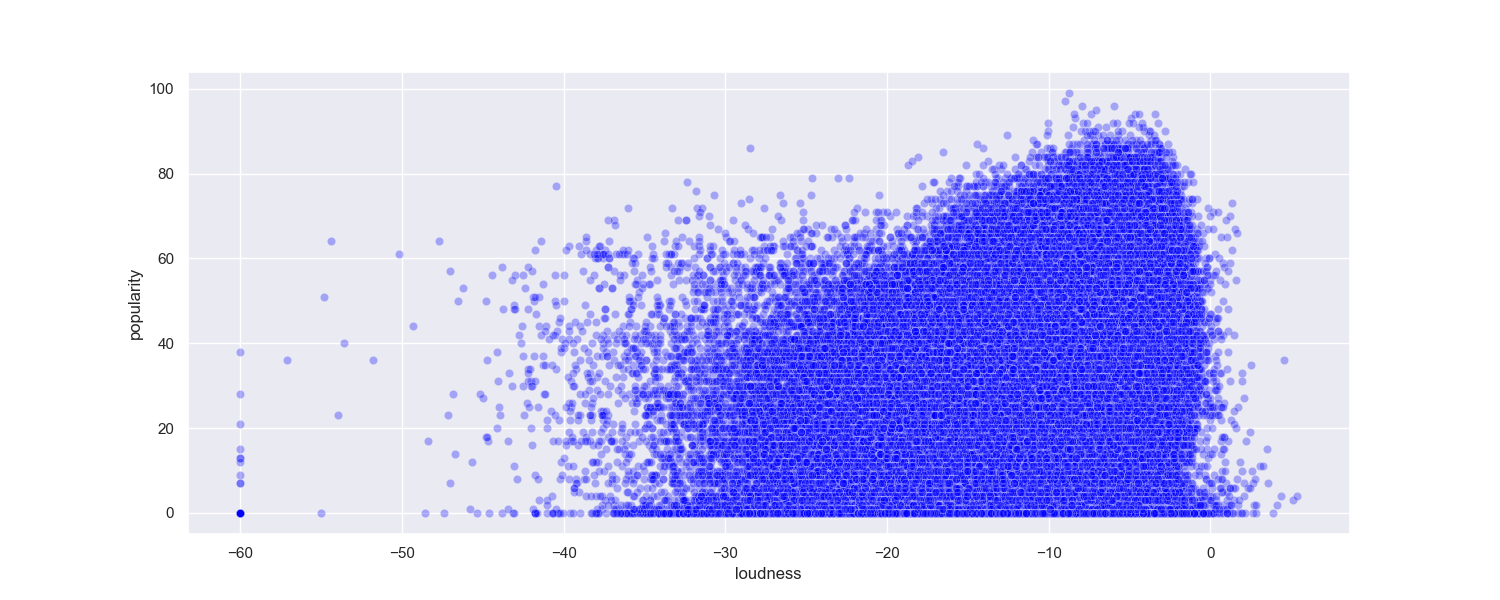
\includegraphics[width=\columnwidth]{images/popularity_loudness_scatterplot.png} \caption{Relación de popularidad e intensidad sonora} \label{fig:relacion popularidad e intensidad sonora} \end{figure}

Además se ha realizado una comparación entre las variables danzabilidad y cuanto se habla en una canción en la \figurename{\ref*{fig:relacion danzabilidad y elocuencia}}. Viéndose que la mayoría de las canciones con mayor nivel de danzabilidad tienen muy poca elocuencia.

\begin{figure}[H] 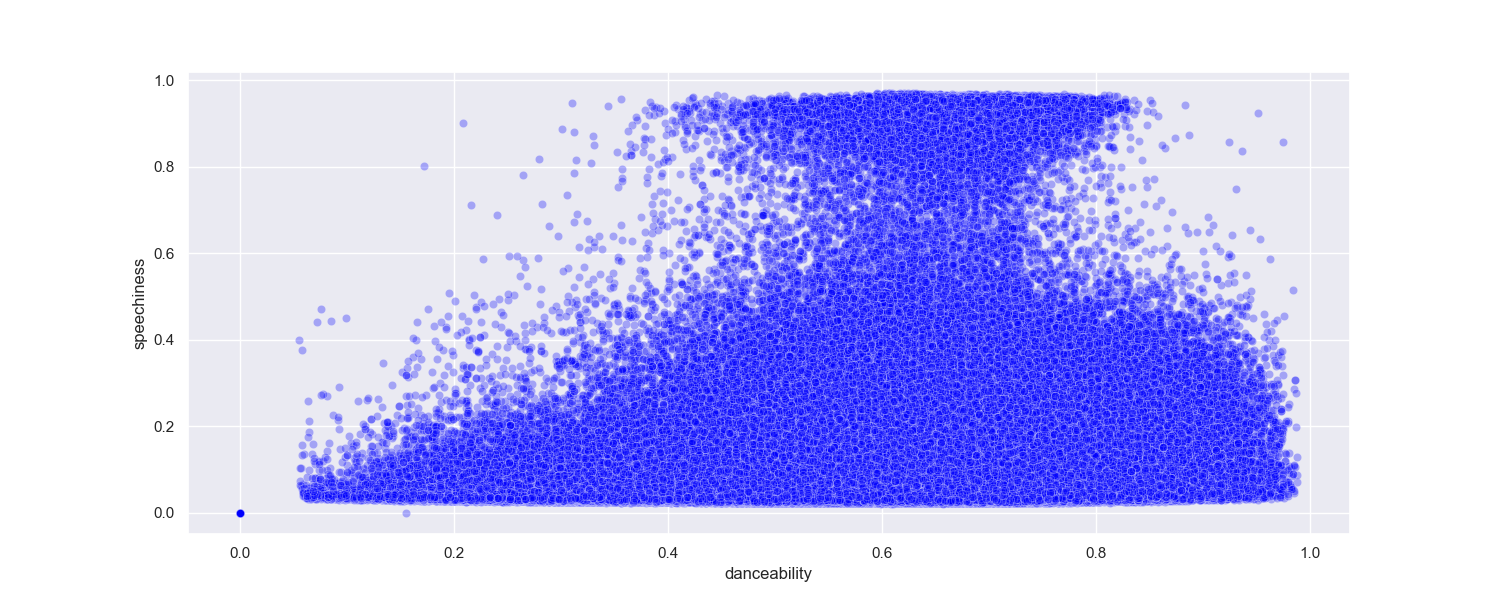
\includegraphics[width=\columnwidth]{images/danceability_speechiness_scatterplot.png} \caption{Relación de danzabilidad y elocuencia} \label{fig:relacion danzabilidad y elocuencia} \end{figure}

Por ultimo se han sacado las relaciones entre varios datos coloreando la popularidad con corte en el 75\% en la \figurename{\ref{fig:relaciones}}. Como se puede ver en la figura, no se pueden ver ninguna relación directa de la popularidad con los datos por lo que no se esperan resultados muy buenos.
\begin{figure}[H] 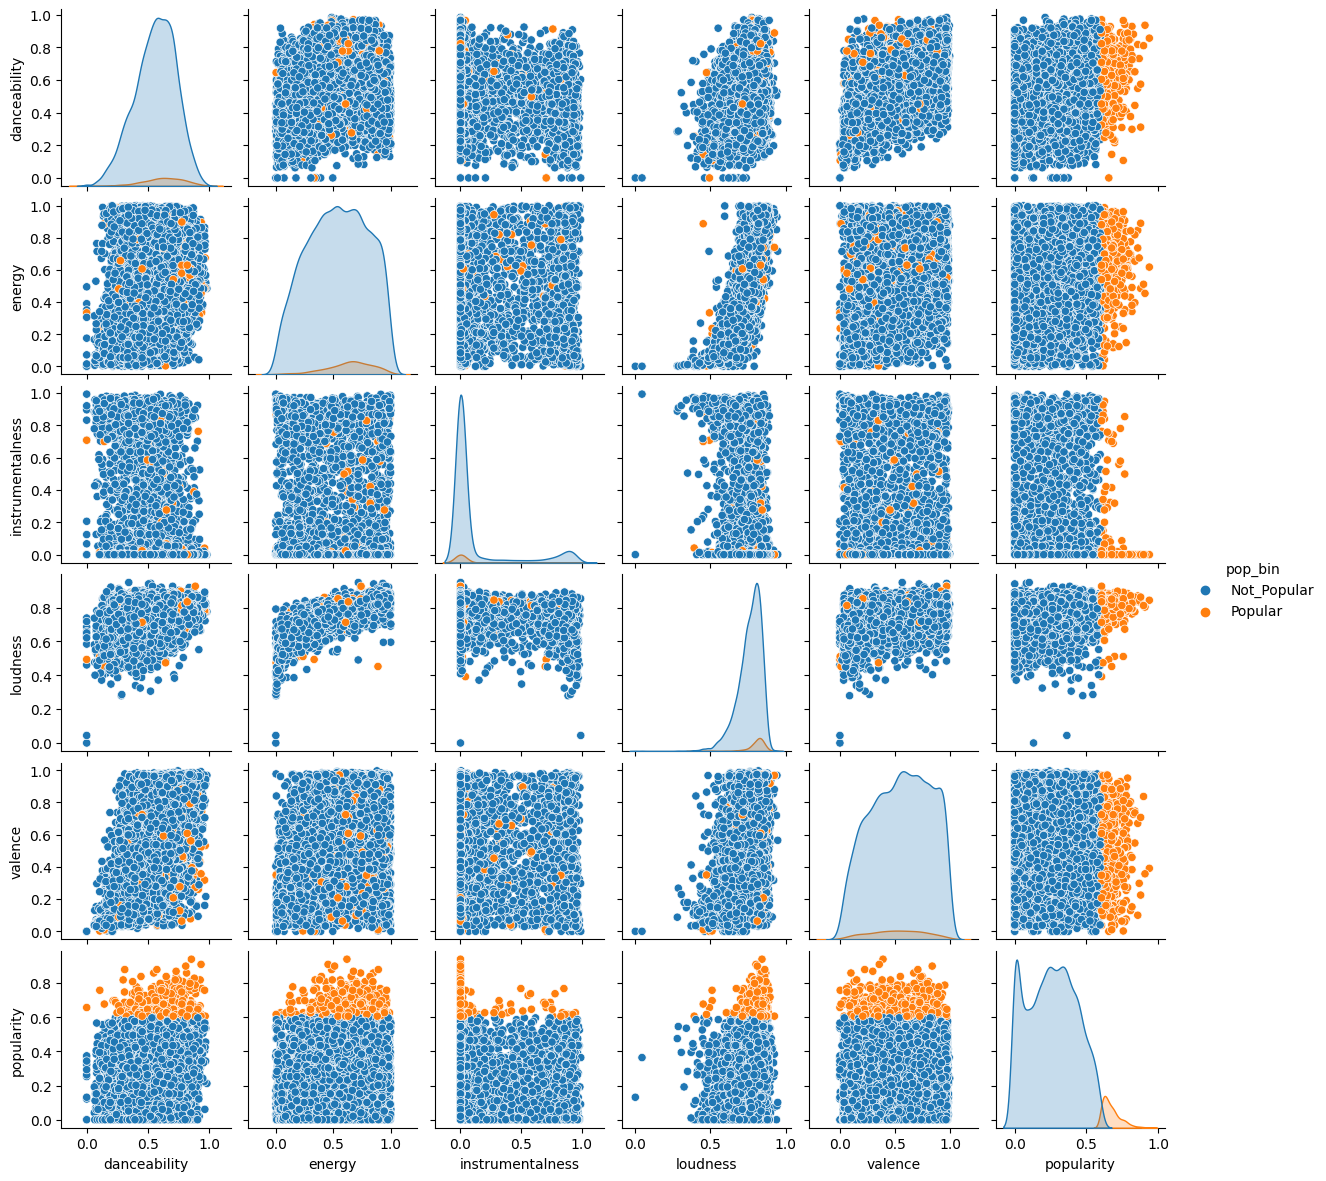
\includegraphics[width=\columnwidth]{images/Relaciones.png} \caption{Relaciones de varios datos} \label{fig:relaciones} \end{figure}




\section{Método}
Primero se realizará un preprocesado de los datos eliminando algunos inservibles, y quedándonos solo con: energy, liveness, tempo, valence, loudness, speechiness, acousticness, danceability, instrumentalness. A continuación se realizara una normalización de los datos que no se encuentran entre 0 y 1 que serian popularity, loudness y tempo.
\subsection{Aprendizaje supervisado}
Para el aprendizaje supervisado primero se dividirá el dataset en dos grupos train y test con una division de 70 a 30. Este aprendizaje se realizará mediante técnicas de regresión. Las elegidas han sido: Simple Linear Regression, KNeighborsRegressor, RandomForestRegressor y una red neuronal de TensorFlow. Una vez entrenado el modelo, este se evaluará con el conjunto de test para obtener diferentes métricas que sirvan como comprobación de que el modelo está funcionando correctamente.
Como mas adelante se explicara, en la sección de resultados, los conseguidos no son lo suficientemente satisfactorios, por lo que se tomara otro enfoque a este problema. En vez de usar regresión, se calificara entre popular y no popular a las canciones, haciendo esta etiquetación a partir de el valor 0.41 de popularidad que se encuentra en el 75\% de los datos. Y seguido de esto se realizara un balanceo de las clases ya que al dividirlo en 75\% y 25\%se han desbalanceado las clases.

\subsection{Aprendizaje no supervisado}
Respecto al aprendizaje no supervisado primero se categorizara el dato de danzabilidad en el 75\% siendo danzable o no danzable las clases que se quedarían. También se balancearan estas clases para tener el mismo numero de cada una. Luego se aplicara primero técnicas reducción de dimensionalidad para intentar sacar algún patron de los datos de clustering, que como se vera en el apartado de resultados no ha sido muy satisfactorio. Por lo que luego se realizara técnicas de clustering en los datos para clasificar la danzabilidad.

\section{Resultados}
\subsection{Aprendizaje supervisado}
Como se explico en la sección del Método de Aprendizaje supervisado primero se ha realizado una regresión con diversos algoritmos consiguiendo los resultados que se pueden ver en el \tablename{\ref{tab:resultados supervisado regresion}}.
Los algoritmos escogidos son:

\begin{itemize}
    \setlength\itemsep{0em}
    \item \textbf{Simple Linear Regression}: método estadístico que busca estimar la relación lineal entre una variable dependiente y una o más variables independientes.
    \item \textbf{KNeighborsRegressor}: estimador basado en los k vecinos más cercanos que predice el objetivo mediante la interpolación local de los objetivos asociados a los vecinos más cercanos en el conjunto de entrenamiento.
    \item \textbf{RandomForestRegressor}: estimador que ajusta un número de árboles de decisión clasificadores en varios subconjuntos del conjunto de datos y utiliza el promedio para mejorar la precisión predictiva y controlar el sobreajuste.
    \item \textbf{Red neuronal TensorFlow}: modelo compuesto por neuronas artificiales que están conectadas entre sí y que se puede implementar con la biblioteca de código abierto TensorFlow.
\end{itemize}

\vspace{5mm}
\begin{table}[H]
    \begin{center}
        \begin{tabular}{| c | c | c | c | }\hline
            Modelo                   & $R^{2}$ & MSE    & MAE    \\ \hline
            Simple Linear Regression & 0.2089  & 0.0264 & 0.1319 \\
            KNeighborsRegressor      & 0.2065  & 0.0290 & 0.1357 \\
            RandomForestRegressor    & 0.3482  & 0.0230 & 0.1199 \\
            Red neuronal TensorFlow  & 0.2986  & 0.0244 & 0.1253 \\ \hline
        \end{tabular}
        \caption{Resultados supervisado regresión}
        \label{tab:resultados supervisado regresion}
    \end{center}
\end{table}

Viendo los resultados obtenidos significa que el modelo no capta bien la relación entre las variables. Por lo tanto, como los resultados obtenidos en $R^{2}$ score son bajos, se puede decir que el modelo de regresión no es bueno y que se debería buscar otro tipo de modelo o mejorar las características de los datos.

Por lo que como explicado anteriormente se pasa a usar diferentes modelos de clasificación con el corte en el 75\%. Los resultados obtenidos se ven en el \tablename{\ref{tab:resultados supervisado clasificacion}}.


\begin{itemize}
    \setlength\itemsep{0em}
    \item \textbf{KNeighborsClassifier}: clasificador que asigna una nueva instancia a la clase más frecuente entre sus k vecinos más cercanos.
    \item \textbf{RandomForestClassifier}: clasificador que construye un conjunto de árboles de decisión aleatorios y combina sus predicciones mediante votación.
    \item \textbf{AdaBoostClassifier}: clasificador que mejora el rendimiento de un algoritmo base mediante la asignación de pesos a las instancias según su dificultad de clasificación.
    \item \textbf{DecisionTreeClassifier}: clasificador que divide el espacio de características en regiones homogéneas según criterios de impureza o ganancia de información.
    \item \textbf{GaussianNB}: clasificador que asume que las características siguen una distribución normal y aplica el teorema de Bayes para estimar las probabilidades posteriores de las clases.
    \item \textbf{MLPClassifier}: clasificador que utiliza una red neuronal multicapa con una o más capas ocultas y una función de activación no lineal.
    \item \textbf{Red neuronal TensorFlow}: clasificador que utiliza una red neuronal definida y entrenada con la librería TensorFlow, que permite una gran flexibilidad y escalabilidad.
\end{itemize}


\vspace{5mm}
\begin{table}[H]
    \begin{center}
        \begin{tabular}{| c | c | c | c | }\hline
            Modelo                  & Accuracy & Precision & F1 score \\ \hline
            KNeighborsClassifier    & 0.6000   & 0.5968    & 0.5944   \\
            RandomForestClassifier  & 0.6894   & 0.6932    & 0.6803   \\
            AdaBoostClassifier      & 0.6791   & 0.6827    & 0.6587   \\
            DecisionTreeClassifier  & 0.6702   & 0.6890    & 0.6112   \\
            GaussianNB              & 0.6449   & 0.7138    & 0.4732   \\
            MLPClassifier           & 0.6761   & 0.7021    & 0.6008   \\
            Red neuronal TensorFlow & 0.6758   & 0.7021    & 0.6475   \\ \hline
        \end{tabular}
        \caption{Resultados supervisado clasificación}
        \label{tab:resultados supervisado clasificacion}
    \end{center}
\end{table}

El modelo \textbf{RandomForestClassifier} obtuvo el mejor desempeño entre los evaluados, con un 69\% de exactitud y un 69\% de precisión. Estos valores, aunque no son óptimos, se explican por la dificultad ya vista en la regresión, que se había anticipado en el análisis previo.

\subsection{Aprendizaje no supervisado}

Como se explico en la sección del Método de Aprendizaje no supervisado, primero se empezara con la prueba de los algoritmos de reducción de dimensionalidad. Los elegidos para la prueba son los siguientes:

\begin{itemize}
    \setlength\itemsep{0em}
    \item \textbf{PCA}: algoritmo que simplifica el problema inicial al proyectar los datos en un espacio de menor dimensionalidad que maximiza la varianza de los datos.
    \item \textbf{TSNE}: algoritmo que preserva la estructura local de los datos al mapearlos en un espacio de dos o tres dimensiones usando una medida de similitud basada en la probabilidad.
    \item \textbf{FastICA}: algoritmo que busca componentes independientes en los datos al maximizar la no gaussianidad de las proyecciones usando una función de contraste.
    \item \textbf{FeatureAgglomeration}: algoritmo que agrupa las características similares en clusters usando una medida de distancia y una técnica de agrupamiento jerárquico.
    \item \textbf{TruncatedSVD}: algoritmo que reduce la dimensionalidad de los datos al aplicar una descomposición en valores singulares truncada que conserva las componentes principales más importantes.
    \item \textbf{NMF}: algoritmo que descompone los datos en dos matrices no negativas que representan las características y los coeficientes de los datos, respectivamente.
\end{itemize}

\begin{figure}[H]
    \centering

    \begin{subfigure}[b]{0.3\columnwidth} 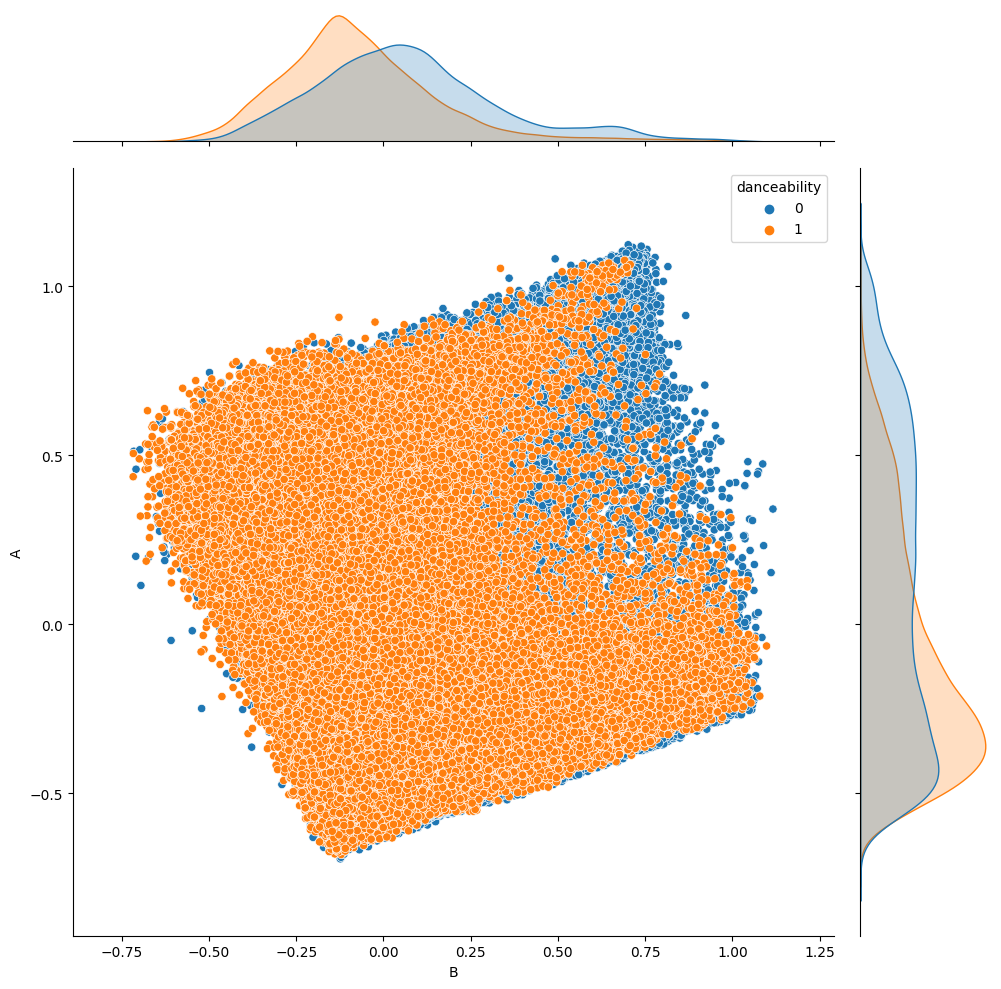
\includegraphics[width=\columnwidth]{images/PCA.png} \caption{PCA} \label{fig:PCA} \end{subfigure}
    \hfill
    \begin{subfigure}[b]{0.3\columnwidth} 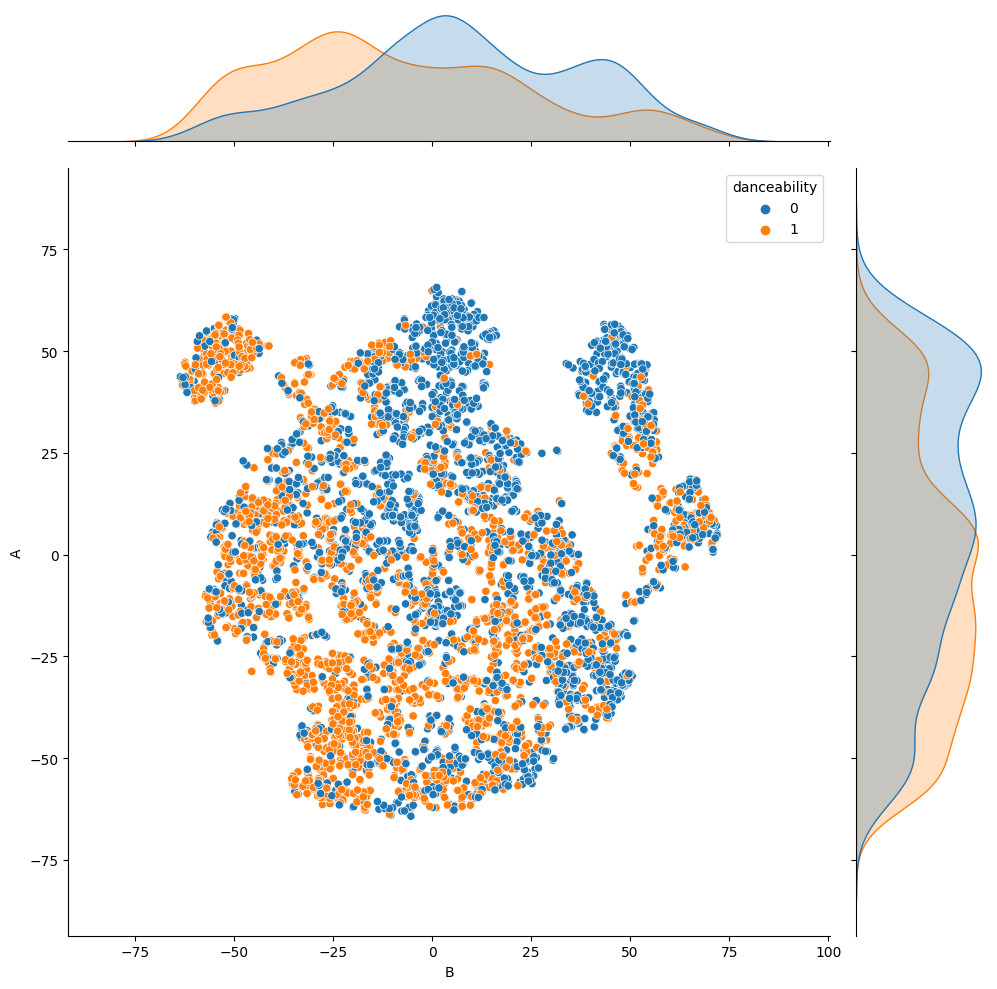
\includegraphics[width=\columnwidth]{images/TSNE.png} \caption{TSNE} \label{fig:TSNE} \end{subfigure}
    \hfill
    \begin{subfigure}[b]{0.3\columnwidth} 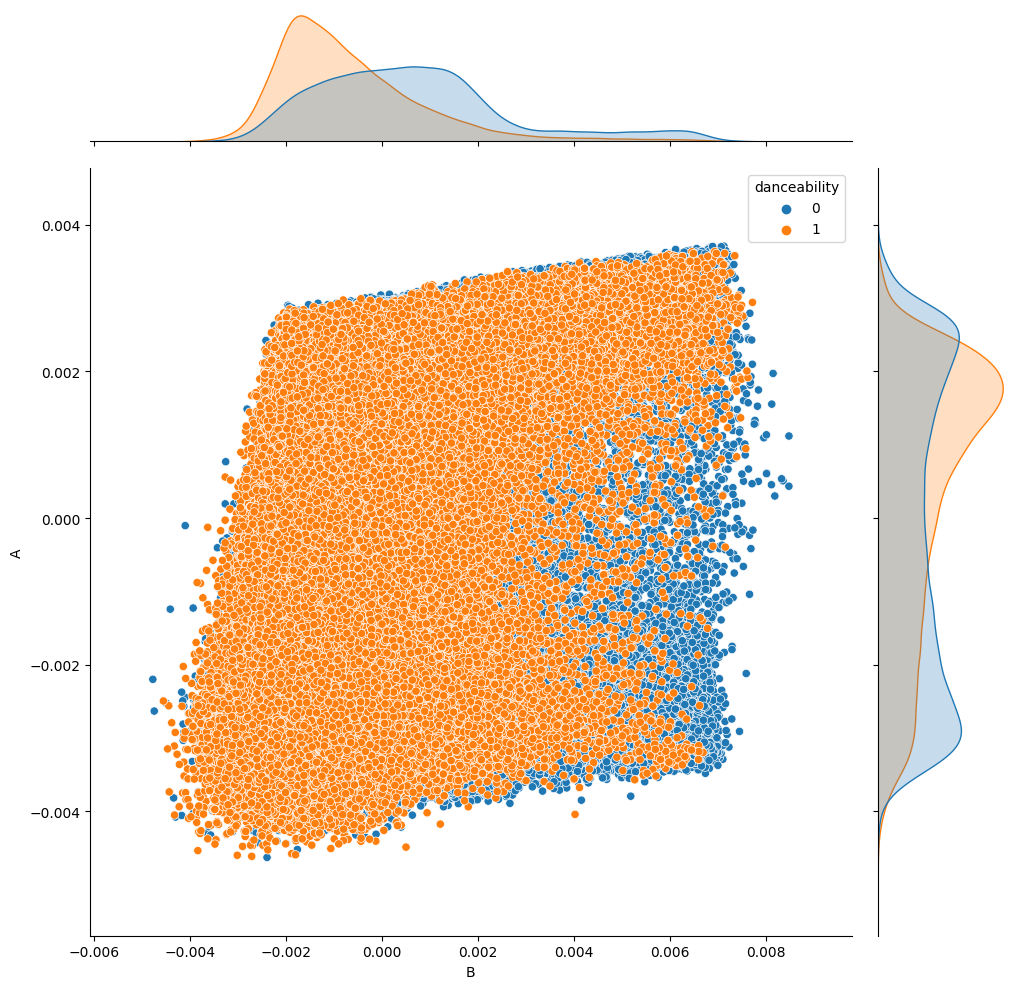
\includegraphics[width=\columnwidth]{images/FastICA.png} \caption{FastICA} \label{fig:FastICA} \end{subfigure}

\end{figure}

\begin{figure}[H]
    \centering

    \begin{subfigure}[b]{0.3\columnwidth} 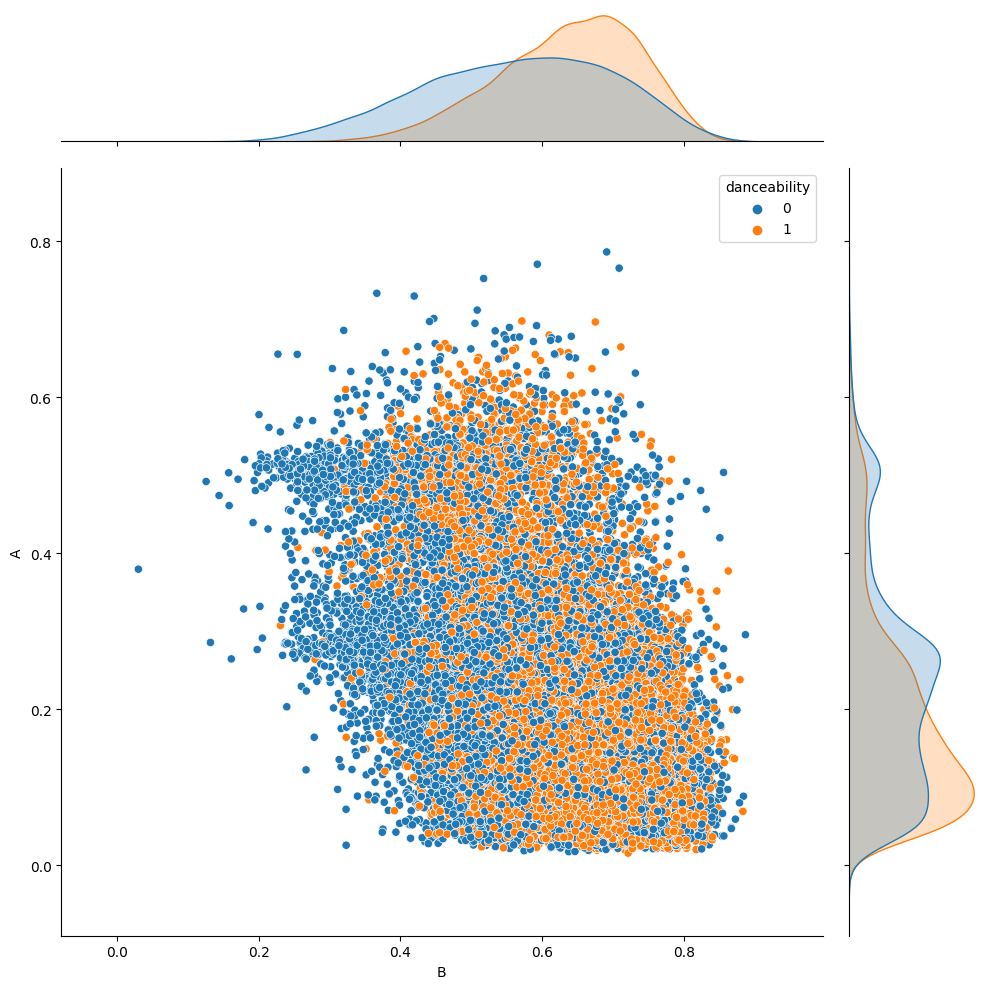
\includegraphics[width=\columnwidth]{images/FeatureAgglomeration.png} \caption{FeatureAgglomeration} \label{fig:FeatureAgglomeration} \end{subfigure}
    \hfill
    \begin{subfigure}[b]{0.3\columnwidth} 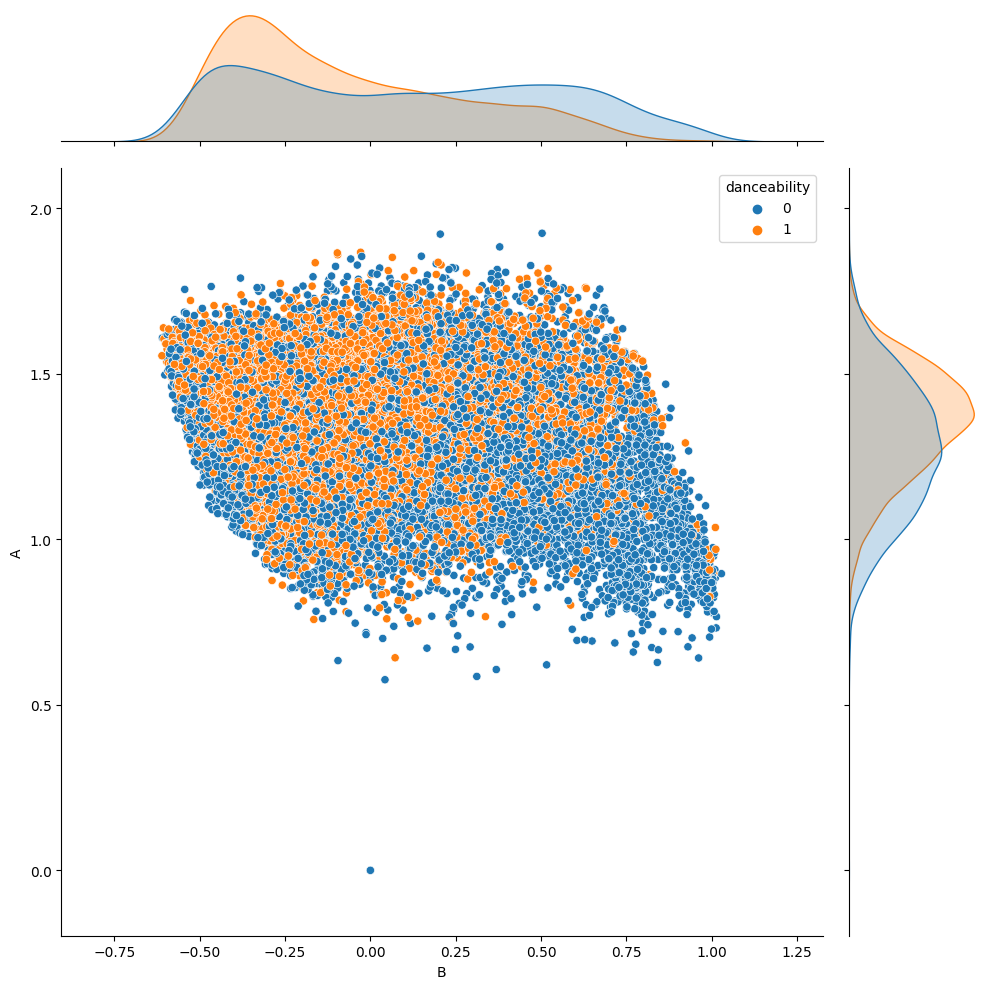
\includegraphics[width=\columnwidth]{images/TruncatedSVD.png} \caption{TruncatedSVD} \label{fig:TruncatedSVD} \end{subfigure}
    \hfill
    \begin{subfigure}[b]{0.3\columnwidth} 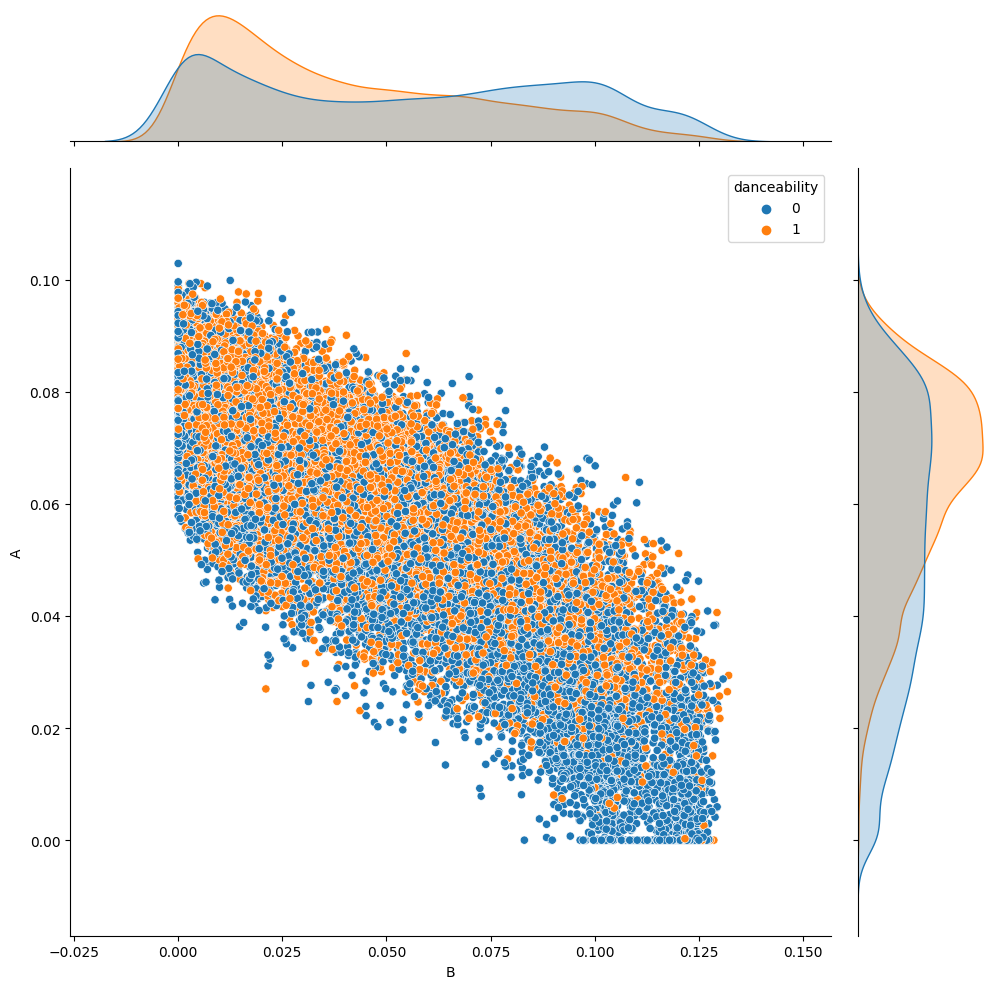
\includegraphics[width=\columnwidth]{images/NMF.png} \caption{NMF} \label{fig:NMF} \end{subfigure}

\end{figure}

La evaluación de las representaciones bidimensionales generadas por los métodos de reducción de dimensionalidad indica que no existe una estructura de grupos o clusters distinguible en los datos originales. Por lo tanto, no se recomienda aplicar ninguna técnica de agrupación basada en la reducción de dimensionalidad.

A continuación, presentaremos los hallazgos obtenidos al aplicar los métodos de agrupamiento o  clustering seleccionados, con sus respectivos análisis. Estos métodos permiten identificar patrones y similitudes entre los datos, según los criterios establecidos previamente.

Los algoritmos elegidos son:
\begin{itemize}
    \setlength\itemsep{0em}
    \item \textbf{MiniBatchKMeans}: algoritmo que divide el conjunto de datos en mini lotes y actualiza los centroides de forma iterativa.
    \item \textbf{SpectralClustering}: algoritmo que utiliza la información de la matriz de afinidad para agrupar los puntos según su similitud espectral.
    \item \textbf{AgglomerativeClustering}: algoritmo jerárquico que fusiona los clusters más cercanos según un criterio de enlace.
    \item \textbf{Birch}: algoritmo que construye un árbol de características compacto y reduce el número de candidatos a clusters.
    \item \textbf{BisectingKMeans}: algoritmo que parte el conjunto de datos en dos subconjuntos y repite el proceso hasta obtener el número deseado de clusters.
\end{itemize}


\vspace{5mm}
\begin{table}[H]
    \begin{center}
        \begin{tabular}{| c | c | c | c | }\hline
            Modelo                  & Accuracy & Precision & Recall \\ \hline
            MiniBatchKMeans         & 0.6052   & 0.4616    & 0.6476 \\
            SpectralClustering      & 0.6057   & 0.4573    & 0.6504 \\
            AgglomerativeClustering & 0.5978   & 0.5202    & 0.6158 \\
            Birch                   & 0.5374   & 0.1137    & 0.7449 \\
            BisectingKMeans         & 0.5988   & 0.5075    & 0.6209 \\
            \hline
        \end{tabular}
        \caption{Resultados no supervisado clustering}
        \label{tab:resultados no supervisado clustering}
    \end{center}
\end{table}
La mayor exactitud obtenida en este estudio fue de un 60,5\%, lo cual indica que el método empleado no es adecuado para resolver el problema planteado. El uso de técnicas de clustering no aportó resultados significativos, por lo que se sugiere explorar otras alternativas. Una posible opción sería aplicar un algoritmo supervisado, o incorporar más variables de entrada para poder detectar posibles patrones en los datos.

\section{Limitaciones}

Este estudio tiene algunas limitaciones que deben tenerse en cuenta al interpretar los resultados. En primer lugar, el conjunto de datos solo contiene canciones de Spotify, lo que puede tener un sesgo de selección hacia ciertos géneros, artistas o regiones. En segundo lugar, los métodos utilizados para el análisis no son perfectos y pueden tener algunos inconvenientes o errores. Los métodos se basan en valores numéricos que cuantifican los atributos acústicos de las canciones, que pueden no captar los aspectos subjetivos o cualitativos de la percepción y apreciación musical. Los métodos también asumen que existe una relación lineal o no lineal entre los atributos acústicos y la popularidad o danzabilidad de las canciones, lo que puede no ser cierto para todos los casos. Los métodos también dependen de la elección de parámetros, como el número de clusters, vecinos o componentes, que pueden afectar el rendimiento o la precisión de los modelos. Por lo tanto, los resultados de este estudio deben tomarse con precaución y no generalizarse a todos los fenómenos musicales.

\section{Conclusiones y Trabajo Futuro}
Este estudio tuvo como objetivo explorar el conjunto de datos de Spotify utilizando técnicas de aprendizaje automático supervisado y no supervisado, para obtener información relevante sobre las canciones y sus características. El aprendizaje supervisado se centró en predecir la popularidad de las canciones en función de sus atributos acústicos, utilizando diferentes modelos de regresión y clasificación. El aprendizaje no supervisado se centró en agrupar las canciones por su danzabilidad en función de sus atributos acústicos, utilizando diferentes métodos de reducción de dimensionalidad y agrupamiento. Los resultados mostraron que ambos tipos de aprendizaje tuvieron un bajo rendimiento y precisión, lo que indica que el conjunto de datos y los métodos no eran adecuados para resolver el problema. También como la música es un arte, algo abstracto, no es posible medir la popularidad de una canción con solo sus métricas tal y como se ha visto con los resultados.
Como trabajo futuro algunas de las posibilidades que se podrían explorar son: utilizar un conjunto de datos más completo y diverso que abarque más canciones, géneros, artistas y regiones; incorporar más variables o características que capturen los aspectos subjetivos o cualitativos de la percepción y apreciación musical, como las letras, el estado de ánimo, el género o el contexto; comparar o combinar diferentes métodos o algoritmos que puedan tener un mejor rendimiento o precisión para predecir la popularidad o la danzabilidad; y explorar otros tipos de técnicas de aprendizaje automático, como el aprendizaje profundo, el procesamiento del lenguaje natural o la visión por computadora, que puedan ofrecer nuevas perspectivas o aplicaciones para el análisis musical.

% use section* for acknowledgment
\bibliographystyle{IEEEtran}
%% you can change the style into any other styles available, I personally love IEEEtran.
\bibliography{citations}
%% to generate references, input the name of your .bib file and cite anywhere in the document.


\end{document}
